\documentclass[a4paper,12pt]{article} 
\usepackage[utf8]{inputenc} % Acentos válidos sin problemas
\usepackage[spanish]{babel} % Idioma
%\usepackage[style=biber]{biblatex}
%\addbibresource{bibliografia.bib}
%\usepackage[
%  backend=biber
%]{biblatex}
\usepackage[backend=biber, style=ieee]{biblatex}
\addbibresource{bibliografia.bib}
\usepackage{csquotes}
%\usepackage{background}
%\setlegtth{\parindent}{2px}
%\phantom{abc}
\usepackage{csvsimple}
\usepackage{filecontents}
%\usepackage{json}
%\usepackage{fancyvrb}


%-----------------------------------INICIO DE PACKETES------------------/
%----------------------------------------------------------------------/|
\usepackage{amsmath}   % Matemáticas: Comandos extras(cajas ecuaciones) |
\usepackage{amssymb}   % Matemáticas: Símbolos matemáticos              |
\usepackage{datetime}  % Agregar fechas                                 |
\usepackage{graphicx}  % Insertar Imágenes                              |
\usepackage{biblatex} % Bibliografía                                   |
\usepackage{multicol}  % Creación de tablas                             |
\usepackage{longtable} % Tablas más largas                              |
\usepackage{xcolor}    % Permite cambiar colores del texto              |
\usepackage{tcolorbox} % Cajas de color                                 |
\usepackage{setspace}  % Usar espacios                                  |
\usepackage{fancyhdr}  % Para agregar encabezado y pie de página        |
\usepackage{lastpage}  %                                                 |
\usepackage{float}     % Flotantes                                      |
\usepackage{soul}      % "Efectos" en palabras                          |
\usepackage{hyperref}  % Para usar hipervínculos                        |
\usepackage{caption}   % Utilizar las referencias                       |
\usepackage{subcaption} % Poder usar subfiguras                         |
\usepackage{multirow}  % Nos permite modificar tablas                   |
\usepackage{array}     % Permite utilizar los valores para multicolumn  |
\usepackage{booktabs}  % Permite modificar tablas                       |
\usepackage{diagbox}   % Diagonales para las tablas                     |
\usepackage{colortbl}  % Color para tablas                              |
\usepackage{listings}  % Escribir código                                |
\usepackage{mathtools} % SIMBOLO :=                                     |
\usepackage{enumitem}  % Modificar items de Listas                      |
\usepackage{tikz}      %                                                |
\usepackage{lipsum}    % for auto generating text                       |
\usepackage{afterpage} % for "\afterpage"s                              |
\usepackage{pagecolor} % With option pagecolor={somecolor or none}|     |
\usepackage{xpatch}    % Color de lineas C & F
%\usepackage{glossaries} %                                             
\usepackage{lastpage}       





%----------------------------------------------------------------------\|
%-----------------------------------FIN--- DE PACKETES------------------\
%\usepackage{listings}
%\lstset{
%  language=Scheme
%}

%--------------------------------/
%-------------------------------/
\usepackage[                 %   |
  headheight=15pt,  %            |
  letterpaper,  % Tipo de pag.   |
  left =1.5cm,  %  < 1 >         |
  right =1.5cm, %  < 1 >         | MARGENES DE LA PAGINA
  top =2cm,     %  < 1.5 >       |
  bottom =1.5cm %  < 1.5 >       |
]{geometry}     %                |
%-------------------------------\
%--------------------------------\

%----------------------------------------------------------------------/
%-------------------Encabezado y Pie de Pagina-----------------------/ |
%--------------------------------------------------------------------\ |
%\fancyhf{}           %                                                |

     %                                                |
%\pagestyle{fancy}

\fancypagestyle{firstpage}{  
  \fancyfoot[L]{\textsc{\textcolor{white}{\small {Fundamentos de Bases de Datos}}}}
  \fancyfoot[C]{}
  \fancyfoot[R]{\textcolor{white}{\thepage\ de \pageref*{LastPage}}} 
  \renewcommand{\footrulewidth}{1.5pt} %     | 
\xpretocmd\footrule{\color{white}}{}{\PatchFailed}
}

\fancypagestyle{fancy}{  

\fancyhead[L]{{\textcolor{white}{2024-1}}} %                         
\fancyhead[R]{\textcolor{white}{}}     % |
\fancyfoot[L]{\textsc{\textcolor{white}{\small {Fundamentos de Bases de Datos}}}}
  \fancyfoot[C]{}
  \fancyfoot[R]{\textcolor{white}{\thepage\ de \pageref*{LastPage}}} 
\renewcommand{\headrulewidth}{1pt} %
\xpretocmd\headrule{\color{white}}{}{\PatchFailed}
\renewcommand{\footrulewidth}{1.5pt} %     | 
\xpretocmd\footrule{\color{white}}{}{\PatchFailed}

}


%--------------------------------------------------------------------\ |
%-------------------Encabezado y Pie de Pagina-----------------------/ |
%------------------------------------------------------------FIN----/

%--------------------------------------------------------------------\ |
%------------------- LISTA DE COLORES -------------------------------/ |
\definecolor{ProcessBlue}{RGB}{0,176,240}
\definecolor{NavyBlue}{RGB}{0,110,184}
\definecolor{Cyan}{RGB}{0,174,239}
\definecolor{MidnightBlue}{RGB}{0,103,49}
\definecolor{ForestGreen}{RGB}{0,155,85}
\definecolor{Goldenrod}{RGB}{255,223,66}
\definecolor{YellowGreen}{RGB}{152,204,112}
\definecolor{Sepia}{RGB}{103,24,0}
\definecolor{Peach}{RGB}{247,150,90}
\definecolor{CarnationPink}{RGB}{242,130,180}
\definecolor{Fuchsia}{RGB}{140,54,140}
\definecolor{WildStrawberry}{RGB}{238,41,103}

\definecolor{Grass}{RGB}{41,238,53}
\definecolor{Meadow}{RGB}{6,243,67}
\definecolor{jellyfish}{RGB}{109,14,130}
\definecolor{rubber}{RGB}{229,27,232}
\definecolor{bullet}{RGB}{225,31,90}
\definecolor{midnight}{RGB}{31,90,225}
\definecolor{sun}{RGB}{241,152,7}
\definecolor{water}{RGB}{16,229,183}
%------------------- LISTA DE COLORES -------------------------------/ |
%----------------------------------------------------------------------/

\usepackage{tikz,times}
\usepackage{verbatim}
\usetikzlibrary{mindmap,trees,backgrounds}

\definecolor{color_mate}{RGB}{255,255,128}
\definecolor{color_plas}{RGB}{255,128,255}
\definecolor{color_text}{RGB}{128,255,255}
\definecolor{color_petr}{RGB}{255,192,192}
\definecolor{color_made}{RGB}{192,255,192}
\definecolor{color_meta}{RGB}{192,192,255}

\lstdefinelanguage{json}{
    basicstyle=\color{white}\normalfont\ttfamily,
    numbers=left,
    numberstyle=\scriptsize,
    stepnumber=1,
    numbersep=8pt,
    showstringspaces=false,
    breaklines=true,
    frame=lines,
    backgroundcolor=\color{black},
    literate=
     *{0}{{{\color{blue!50!white}0}}}{1}
      {1}{{{\color{blue!50!white}1}}}{1}
      {2}{{{\color{blue!50!white}2}}}{1}
      {3}{{{\color{blue!50!white}3}}}{1}
      {4}{{{\color{blue!50!white}4}}}{1}
      {5}{{{\color{blue!50!white}5}}}{1}
      {6}{{{\color{blue!50!white}6}}}{1}
      {7}{{{\color{blue!50!white}7}}}{1}
      {8}{{{\color{blue!50!white}8}}}{1}
      {9}{{{\color{blue!50!white}9}}}{1}
      {:}{{{\color{orange!70!black}{:}}}}{1}
      {,}{{{\color{orange!70!black}{,}}}}{1}
      {\{}{{{\color{red!60!black}{\{}}}}{1}
      {\}}{{{\color{red!60!black}{\}}}}}{1}
      {[}{{{\color{red!70!white}{[}}}}{1}
      {]}{{{\color{red!70!white}{]}}}}{1},
}

\begin{document}%----------------------INICIO DOCUMENTO------------|
%------------------------------------------------------------------|
\pagecolor{black}
\color{white}

\thispagestyle{firstpage} % Aplicar estilo de primera página
\noindent
%%%%%%%%%%%%%%%%%%%%%%%%%%%%%%%%%%%%%%%%%%%%%%%%%%%%%%%%%%%%%%%%%%%%%%%%%%%%%%
\large\textbf{Facultad de Ciencias} \\
Fundamentos de Bases de Datos \hfill semestre: 2024-1 \\
\textsc{SILVA HUERTA MARCO}   \hfill No.Cuenta: 316205326    \\
11 de Septiembre de 2023      \hfill \textbf{Practica \#02}    \\
\noindent\rule{7.3in}{2.8pt}
%%%%%%%%%%%%%%%%%%%%%%%%%%%%%%%%%%%%%%%%%%%%%%%%%%%%%%%%%%%%%%%%%%%%%%%%%%%%%%

\begin{center}
\Large{Modelos de datos}
\end{center}



\subsection*{Ejercicio 1}

Modelo semiestructurado

\textcolor{sun}{Deberás leer el archivo csv de la práctica 1 y pasarlo a alguna estructura del modelo
semiestructurado (json, xml, html etcétera), recomiendo json por ser el más usado.}


\subsubsection*{Archivo CSV}

\begin{filecontents*}{productos.csv}
    ID,Nombre,Categoria,Precio,Cantidad en Existencia
    AMOANA,Amoxicilina,Antibióticos,150.0,24
    IBUAOS,Ibuprofeno,Analgésicos,50.0,50
    PARAOS,Paracetamol,Analgésicos,30.0,100
    OMEOOS,Omeprazol,Otros,20.0,30
    ASPAOS,Aspirina,Analgésicos,40.0,60
    VITAOS,Vitaminas,Alimentos,15.0,200
    AGUBAS,Agua Mineral,Bebidas,5.0,120
    CREHTE,Crema Hidratante,Desinflamantes,25.0,40
    JABOOS,Jabón de Manos,Otros,8.0,75
    SUEBAS,Suerox,Bebidas,20.0,20
    SUEBAS,Suerox,Bebidas,15.5,10
\end{filecontents*}

\csvautotabular{productos.csv}

\subsubsection*{Archivo JSON}

%\jsonfile{productos.json}
\thispagestyle{fancy} % Aplicar estilo de primera página
\begin{lstlisting}[language=json]
    {
        [
            {
              "ID": "AMOANA",
              "Nombre": "Amoxicilina",
              "Categoria": "Antibioticos",
              "Precio": 150.0,
              "Cantidad en Existencia": 24
            },
            {
              "ID": "IBUAOS",
              "Nombre": "Ibuprofeno",
              "Categoria": "Antibioticos",
              "Precio": 50.0,
              "Cantidad en Existencia": 50
            },
            {
              "ID": "OMEOOS",
              "Nombre": "Omeprazol",
              "Categoria": "Otros",
              "Precio": 20.0,
              "Cantidad en Existencia": 30
            },
            {
              "ID": "ASPAOS",
              "Nombre": "Aspirina",
              "Categoria": "Analgesicos",
              "Precio": 40.0,
              "Cantidad en Existencia": 60
            },
            {
              "ID": "VITAOS",
              "Nombre": "Vitaminas",
              "Categoria": "Alimentos",
              "Precio": 15.0,
              "Cantidad en Existencia": 200
            },
            {
              "ID": "AGUBAS",
              "Nombre": "Agua Mineral",
              "Categoria": "Bebidas",
              "Precio": 5.0,
              "Cantidad en Existencia": 120
            },            
            {
              "ID": "CREHTE",
              "Nombre": "Crema Hidratante",
              "Categoria": "Desinflamantes",
              "Precio": 25.0,
              "Cantidad en Existencia": 40
            },
            {
              "ID": "SUEBAS",
              "Nombre": "Suerox",
              "Categoria": "Bebidas",
              "Precio": 15.5,
              "Cantidad en Existencia": 10
            },
            {
              "ID": "LLAOOS",
              "Nombre": "Llavero",
              "Categoria": "Otros",
              "Precio": 15.5,
              "Cantidad en Existencia": 90
            },
            {
              "ID": "PALAOS",
              "Nombre": "Paletas",
              "Categoria": "Alimentos",
              "Precio": 12.0,
              "Cantidad en Existencia": 30
            }
          ]          
    }
\end{lstlisting}
\thispagestyle{fancy} % Aplicar estilo de primera página

\newpage
\thispagestyle{fancy} % Aplicar estilo de primera página

\subsection*{Ejercicio 2}

Modelo relacional

\textcolor{sun}{Basándote en las figuras 1.2 y 2.1 diseña un esquema de base de datos y coloca algunos
registros de ejemplo sobre un universo de discurso de tu elección.}

\begin{center}
    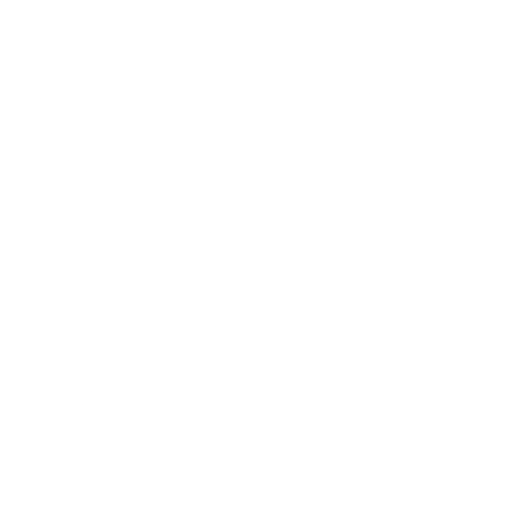
\includegraphics[scale = .6]{ejercico02.png}
\end{center}



\subsection*{Ejercicio 3}

Completa el modelo con los siguientes aspectos:

\begin{enumerate}
    \item \textcolor{sun}{¿Qué tipo de información adicional y restricciones podrías representar en este
    esquema? Inventa al menos 5 restricciones y agrega al menos 5 campos distribuidos
    en distintas tablas, también si lo consideras necesario, puedes agregar una tabla
    adicional.}

    \begin{itemize}
      \item \textbf{Restricción de Unicidad en Departamentos:} Agregar una restricción única para el campo `Departamento` en la tabla de `Departamento` para garantizar que no haya departamentos con el mismo nombre.
      
      \item \textbf{Fecha de Inicio en Secciones:} Agregar un campo `Fecha de Inicio` en la tabla de `Sección` para registrar la fecha en que una sección comienza.
      
      \item \textbf{Restricción de Calificaciones:} Agregar una restricción de rango en la tabla de `Calificaciones` para garantizar que las calificaciones estén dentro de un rango específico (por ejemplo, A, B, C, D, F).
      
      \item \textbf{Restricción de Edad en Estudiantes:} Agregar un campo `Fecha de Nacimiento` en la tabla de `Estudiante` para calcular automáticamente la edad y aplicar una restricción de edad mínima (por ejemplo, 18 años).
      
      \item \textbf{Tabla de Profesores:} Agregar una nueva tabla llamada `Profesor` que almacene información sobre los profesores, como su nombre, número de identificación y departamento al que están asignados. Esta tabla estaría relacionada con la tabla de `Sección` para identificar quién imparte cada sección.
    \end{itemize}
 
    \subsubsection*{Tabla agregada}

    \begin{table}[h]
      \centering
      \caption{\textcolor{white}{Tabla Profesor}}
      \label{tabla_profesor}
      \textcolor{white}{
      \begin{tabular}{|c|c|c|}
      \hline
          Nombre & Numero\_Identificacion & Departamento \\ \hline
          Profesor X & 12345 & CS \\ \hline
          Yoda & 67890 & MATH \\
      \hline
      \end{tabular}
      }
    \end{table}
    

    \item \textcolor{sun}{Menciona al menos 3 usuarios de tu base de datos, define los privilegios que cada
    uno tendría en la BD y describe el tipo de información que cada uno de ellos
    utilizaría.}

    \begin{itemize}
      \item \textbf{Administrador de la Base de Datos:} Los administradores tienen privilegios completos sobre la base de datos. Puede crear, modificar y eliminar tablas, así como otorgar permisos a otros usuarios. Su función es mantener la integridad y la estructura de la base de datos.
    
      \item \textbf{Profesor:} Los profesores tienen acceso a la información de las tablas \textit{Sección} y \textit{Calificaciones}. Tienen permiso para ver y actualizar las calificaciones de los estudiantes en las secciones que imparten. También pueden consultar información sobre las secciones que están a cargo.      
    
      \item \textbf{Departamento de Admisiones:} Ellos tiene acceso a la tabla \textit{Estudiante} para registrar nuevos estudiantes en la base de datos. También puede consultar información sobre los departamentos y cursos ofrecidos.          
    \end{itemize}

  
\end{enumerate}


\section*{Cuestionario}

\begin{enumerate}
    \item \textcolor{sun}{¿Cuáles son las 4 principales características de los modelos orientados a objetos?}
    \item \textcolor{sun}{¿Cuáles son las 4 principales propiedades de una relación?}
    \item \textcolor{sun}{¿Cuál es la principal diferencia entre el modelo entidad relación y el modelo
    semiestructurado?}
    \item \textcolor{sun}{Nombra 3 ejemplos en el cual se utilice el modelo orientado a objetos.}
    \item \textcolor{sun}{Nombra 3 ejemplos en el cual se utilice el modelo entidad relación.}
    \item \textcolor{sun}{Nombra 3 ejemplos en el cual se utilice el modelo semiestructurado.}
\end{enumerate}

\newpage
\thispagestyle{fancy} % Aplicar estilo de primera página

\section*{Tablas de referencia}

\begin{table}[h]
    \centering
    \caption{\textcolor{white}{Tabla Estudiante}}
    \label{tabla_estudiante}
    \textcolor{white}{
    \begin{tabular}{|c|c|c|c|} 
    \hline
        Nombre & Numero\_Estudiante & Clase & Departamento \\ \hline
        Juan & 4 & 1 & CS \\ \hline
        Luis & 17 & 2 & CS \\ 
    \hline
    \end{tabular}
    }
\end{table}
\begin{table}[h]
    \centering
    \caption{\textcolor{white}{Tabla Curso}}
    \label{tabla_curso}
    \textcolor{white}{
    \begin{tabular}{|c|c|c|c|}
    \hline
    Nombre\_Curso & Numero\_Curso & Horas & Departamento \\
    \hline
        Introducción a Computación & CS1310 & 4 & CS \\
        Estructura de datos & CS3320 & 4 & CS \\
        Matemáticas Discretas & MATH2410 & 3 & MATH \\
        Bases de datos & CS3380 & 3 & CS \\
    \hline
    \end{tabular}
    }
\end{table}
\begin{table}[h]
    \centering
    \caption{\textcolor{white}{Tabla Sección}}
    \label{tabla_seccion}
    \textcolor{white}{
    \begin{tabular}{|c|c|c|c|}
    \hline
        Numero\_Curso & Semestre & Año & Instructor \\ \hline
        MATH2410 & Otoño & 07 & Smith \\
        CS1310 & Primavera & 08 & Lucas \\
    \hline
    \end{tabular}
    }
\end{table}
\begin{table}[h]
    \centering
    \caption{\textcolor{white}{Tabla Calificaciones}}
    \label{tabla_calificaciones}
    \textcolor{white}{
    \begin{tabular}{|c|c|c|}
    \hline
        Número\_Estudiante & ID\_Seccion & Calificacion \\ \hline
                2      &     1       & A \\
                1      &     2       & B \\
    \hline
    \end{tabular}
    }
\end{table}
\begin{table}[h]
    \centering
    \caption{\textcolor{white}{Tabla Prerrequisitos}}
    \label{tabla_prerrequisitos}
    \textcolor{white}{
    \begin{tabular}{|c|c|}
    \hline
        Numero\_Curso & Numero\_Prerrequisito \\ \hline
        CS1310        & CS3320 \\
    \hline
    \end{tabular}
    }
\end{table}
    


    
%\newpage
%\thispagestyle{fancy} % Aplicar estilo de primera página

%\printbibliography


%\newpage
%\thispagestyle{fancy} % Aplicar estilo de primera página
%\NoBgThispage % Quita el fondo de la pagina

%-----------------------------------------------------------------|
\end{document}%----------------------FIN DEL DOCUMENTO------------| 